\chapter{The Proposed Solution}\pagestyle{fancy}\setlength{\parindent}{3em}
\label{chap:proposed-solution}

The solution is an image processing pipeline that would extract from the side picture of a tire the specifications written on it. These specifications are present in the form of embossed letters on the tire's exterior walls.

The system's input data are photos taken with a Cannon EOS 1300D that has a resolution of 5184 by 3456 pixels and a lens (TODO: specificatiile lentilei). While taking the pictures, the distance from the lens to the tire's side was approximately (TODO: distanta aproximativa pana la cauciuc cand fac poze). While capturing the images, I was careful to catch the entire wheel in the image because detecting half wheels or arcs would have proven difficult. One more adjustment I did was the camera placement in regards to the wheel's axle. I decided to be approximately in line with it in order for the wheel to appear circular in the image. If I wouldn't have done so, the tire would have had an oval shape. By controlling the distance between the camera and the wheel, as  well as the camera position in regards to the wheel's axle, I consider I will be able to detect the tire in the image more reliably.

By desiring to not have a complex setup and not require supplementary light sources, the images were taken using the ambient light. This proved to increase the problem's difficulty quite considerably when it came to detecting the regions of text, because the contrast between the embossed letters and the background image got even smaller. Multiple approaches were considered in TODO section 3.2 Text Detection and in the end one proved fruitful in delivering acceptable results.

The system's steps are described in the following sections:

\section{Tire Unwrapping}\label{sec:tire-unwrapping}

As a first step, I wanted to extract only the tire from the input image. This would help because the information I am interested in is located on it. I would also like to unwrap the tire from its disk shape (a circle with a smaller circle as a hole inside of it) into a rectangular one in order to have the writing from left to right rather than in all directions like if it was in a circle.

To better explain how this was accomplished, this step was split in multiple sub-steps:

%%%%%%%%%%%%%%%%%%%%%%%%%%%%%%%%%%%%%%%%%%%%%%%%%%%%%%%%%%%%%%%%%%%%%%%%%%%%%%%%%%%%%%%%%%%%%%%%%%%%%%%%%%%%%%%%%%%%%%%%
\subsection{Circle Detection}

I detect where in the image are the circles representing the outer and inner borders of the tire and get their center’s coordinates. The two detected circles might not have a common center because of the imperfections in taking the images, but I account and try to correct for that through a series of heuristics.

Because this is the beginning of the pipeline, I introduced a step to \hyperref[subsubsec:equalization]{equalization} the images and have some independence from the lighting conditions. Then I detected the first circles in the image using TODO: \hyperref[subsubsec:hough_circle_transform]{Hough Circle Transform} and filtered its output through a series of TODO: heuristics.

%%%%%%%%%%%%%%%%%%%%%%%%%%%%%%%%%%%%%%%%%%%%%%%%%%%%%%%%%%%%
%%% a) EQUALIZATION                                      %%%
%%%%%%%%%%%%%%%%%%%%%%%%%%%%%%%%%%%%%%%%%%%%%%%%%%%%%%%%%%%%
\subsubsection{Equalization}
\label{subsubsec:equalization}

\paragraph*{Accomplishes:}\mbox{}\par
Lighting conditions are not controlled and this might result in low contrast in some areas of the image. Here we ensure a constant contrast across the entire image and that the entire histogram is used. This increases the robustness of the overall system.

\paragraph*{Reasoning:}\mbox{}\par
The pixel in a black and white image is a representation of how bright that particular part of the image should be (0 is for no light and 255 is for maximum brightness on a 8 bit sensor). If we take a photo in broad daylight, the values of all the pixels could all be over 200 lets say. The image would appear as being washed-out and lacking details (Figure 5a). If the photo is taken in a dark environment and all pixel values are under 100, the image appears again quite dark and lacking detail (Figure 5b). A solution is to use the space that remained unused in pixel values and stretch the existing pixel values to also cover those, thus increasing the contrast of the image and its level of detail (Figure 5c). This action is called equalization and can be used to enhance the contrast in an image. Furthermore, it spreads the pixel values across their entire value range so that a under-light and an over-light picture's histogram would look similar. The histogram is a plot that has on the $X$ axis all possible pixel values and on the $Y$ axis the number of times that value appears in an image.

TODO: Figure 5 (a, b, c)

A deviation from this standard equalization is Adaptive Histogram Equalization (AHE) that is not applied on the entire image and just on a small portion of it. When calculating the new value for a pixel, only a neighborhood around it is taken into consideration. Thus method while useful in bringing more contrast in to an image that has lighter and darker regions, it also increases the noise in the image. To counteract this, Contrast Limited AHE (CLAHE) was created. The addition is that it has a clipping upper limit and redistributes the pixels that appear too often in the image into another ranges.

\paragraph*{Algorithm:}\mbox{}\par

CLAHE, described in pseudo-code in Algorithm \ref{alg:CLAHE} in accordance to the implementation found in \cite{site:CLAHE_code} and the explanation in the paper \cite{article:CLAHE_explanation}.

On $line 1$ we split the image in multiple cells of size $k$ by $k$ because CLAHE is an adaptive algorithm.
Then, for each of the cells we calculate their histogram to find out how many different pixel values they contain ($N_{gray}$). To perform the clipping, we need to calculate a few things:

$N_{avg} \gets (k \times k) \div N_{gray}$, that is the number of pixels in the cell divided by how many pixel values are present in the cell;

$N_{CL} \gets cl \times N_{avg}$, the clipping limit calculated based on input parameter $cl$;

$N_{\Sigma\_clip} \gets \sum_{i=0}^{N_{gray}} max(0, H_s[i] - N_{CL})$, is the number of pixels that need to be clipped;

$N_{avg\_gray} \gets N_{\Sigma\_clip} \div N_{gray}$, is how many pixels in average we will modify in addition to have a certain value.

Then, we iterate through all the pixel values in the histogram and create a new one. If the pixel count is $\geq$ than $N_{CL}$, we will clip that pixel value. Else, we will add to the pixel count $N_{avg\_gray}$ and if we exceed the clipping limit, we floor to it and take note of this in the form of $N_remain$. After this step, the histogram would look like in figure \ref{fig:CLAHE_hist}.

\begin{figure}[h!]
    \centering
    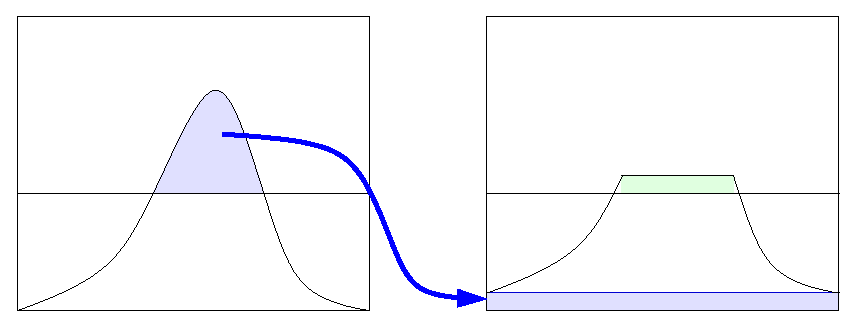
\includegraphics[width=0.4\columnwidth]{img/algos/Clahe-redistribution.eps}
    \caption{the histogram after first clipping, source: TODO wikipedia}
    \label{fig:CLAHE_hist}
\end{figure}

% TODO: figure source https://en.wikipedia.org/wiki/Adaptive_histogram_equalization

The limit we excede with will be redistributed after this on $line 5$. Here, we go through the pixel values in the histogram again and at a simmilary random step we add one more pixel to the count that overflowed earlyer. The step is computed by the formula: $step \gets N_{gray} \div N_{remain}$.

Before starting to compute the next cell, we adjust the current one acoording to the new histogram we just computed: $H_{res}$.

After all the cels were modified and equalized, we can stisch them back together. But because we had a cell by cell approach to calculating the histogram, border pixels might have very different values. This is why an extra step of bilinear interpolation is performed on the border pizels of each of the cells.

\begin{algorithm}[t]
\caption{CLAHE}\label{alg:CLAHE}
\begin{algorithmic}[1]
    \Require $img$ be a $X\times X$ matrix; $cl \epsilon [0, 1]$; $k$

    \Ensure $k \mid X$

    \State $S \gets $ ($img$ split into $k\times k$ cells)

    \For {$s$ in $S$}
        \State $H_s \gets histogram(s)$
        \State $H_{res}, N_{remain} \gets clip(H_s, cl)$
        % \State $N_{avg} \gets (k \times k) \div N_{gray}$
        % \State $N_{CL} \gets N_{clip} \times N_{avg}$
        % \State $N_{\Sigma\_clip} \gets \sum_{i=0}^{N_{gray}} max(0, H_s[i] - N_{CL})$
        % \State $N_{avg\_gray} \gets N_{\Sigma\_clip} \div N_{gray}$
        % \State $N_{remain} \gets N_{\Sigma\_clip}$
        % \For {$i=0:+1:N_{gray}$}
        %     \If {$H_s[i] > N_{CL}$}
        %         \State $H_{res}[i] \gets N_{CL}$
        %     \ElsIf {($H_s[i] + N_{avg\_gray}) > N_{CL}$}
        %         \State $N_{remain} \gets N_{remain} - (N_{CL} - H_s[i])$
        %         \State $H_{res}[i] \gets N_{CL}$
        %     \Else
        %         \State $N_{remain} \gets N_{remain} - N_{avg\_gray}$
        %         \State $H_{res}[i] \gets H_s[i] + N_{CL}$
        %     \EndIf
        % \EndFor

        \State $H_{res} \gets redistribute(H_{res}, N_{remain})$
        % \While {$N_{remain} > 0$}
        %     \State $step \gets N_{gray} \div N_{remain}$
        %     \For {$i=0:step:N_{gray}$}
        %         \If{$H_{res}[i] < N_{CL}$}
        %             \State $H_{res}[i] \gets H_{res}[i] + 1$
        %             \State $N_{remain} \gets N_{remain} - 1$
        %         \EndIf
        %     \EndFor
        % \EndWhile

        \State $s \gets adjust\_cell(s, H_{res})$
    \EndFor

    \State $img \gets$ interpolate cells $S$

\end{algorithmic}
\end{algorithm}

\paragraph*{Results:}\mbox{}\par
After equalization is applied, if the input image's histogram looked like TODO: Figure, now it looks like TODO: Figure.

%%%%%%%%%%%%%%%%%%%%%%%%%%%%%%%%%%%%%%%%%%%%%%%%%%%%%%%%%%%%
%%% b) HOUGH CIRCLE TRANFORM                             %%%
%%%%%%%%%%%%%%%%%%%%%%%%%%%%%%%%%%%%%%%%%%%%%%%%%%%%%%%%%%%%

\subsubsection{Hough Circle Transform}
\label{subsubsec:hough_circle_transform}

\paragraph*{Accomplishes:}\mbox{}\par

\paragraph*{Reasoning:}\mbox{}\par

\paragraph*{Algorithm:}\mbox{}\par

\paragraph*{Results:}\mbox{}\par

%%%%%%%%%%%%%%%%%%%%%%%%%%%%%%%%%%%%%%%%%%%%%%%%%%%%%%%%%%%%
%%% c) HEURISTICS                                        %%%
%%%%%%%%%%%%%%%%%%%%%%%%%%%%%%%%%%%%%%%%%%%%%%%%%%%%%%%%%%%%

\subsubsection{Heuristics}
\label{subsubsec:heuristics}

\paragraph*{Accomplishes:}\mbox{}\par

\paragraph*{Reasoning:}\mbox{}\par

\paragraph*{Algorithm:}\mbox{}\par

\paragraph*{Results:}\mbox{}\par



%%%%%%%%%%%%%%%%%%%%%%%%%%%%%%%%%%%%%%%%%%%%%%%%%%%%%%%%%%%%%%%%%%%%%%%%%%%%%%%%%%%%%%%%%%%%%%%%%%%%%%%%%%%%%%%%%%%%%%%%
\subsection{Convert to Polar Coordinates}


\section{Text Detection}\label{sec:text-detection}

\subsection{Segmentation}

\subsection{Segment Binarization}

\subsection{Filtering for Text}

\subsection{Voting}

\section{Text Recognition}\label{sec:text-recognition}


%%%%%%%%%%%%%%%%%%%%%%%%%%%%%%%%%%%%%%%%%%%%%%%%%%%%%%%%%%%%
%%% x) TEMPLATE                                          %%%
%%%%%%%%%%%%%%%%%%%%%%%%%%%%%%%%%%%%%%%%%%%%%%%%%%%%%%%%%%%%

% TODO: remove
\subsubsection{TEMPLATE}
\label{subsubsec:TEMPLATE}

\paragraph*{Accomplishes:}\mbox{}\par

\paragraph*{Reasoning:}\mbox{}\par

\paragraph*{Algorithm:}\mbox{}\par

\paragraph*{Results:}\mbox{}\par
